%%%%%%%%%%%%%%%%%%%% book.tex %%%%%%%%%%%%%%%%%%%%%%%%%%%%%
%
% sample root file for the chapters of your "monograph"
%
% Use this file as a template for your own input.
%
%%%%%%%%%%%%%%%% Springer-Verlag %%%%%%%%%%%%%%%%%%%%%%%%%%


% RECOMMENDED %%%%%%%%%%%%%%%%%%%%%%%%%%%%%%%%%%%%%%%%%%%%%%%%%%%
\documentclass[pdftex,12pt, oneside]{book}
 
% choose options for [] as required from the list
% in the Reference Guide, Sect. 2.2
%\usepackage[paperwidth=8.5in, paperheight=13in]{geometry} %Folio
\usepackage[paperwidth=8.27in, paperheight=11.69in]{geometry} %A4

\usepackage{makeidx}         % allows index generation
\usepackage{graphicx}        % standard LaTeX graphics tool
                             % when including figure files
\usepackage[bottom]{footmisc}% places footnotes at page bottom
\usepackage[bahasa]{babel}
\usepackage{enumerate}
\usepackage{paralist}
\usepackage{float}
\usepackage{gensymb}  
\usepackage{listings}
\usepackage{color}
\renewcommand{\baselinestretch}{1.5}

\newcommand{\HRule}{\rule{\linewidth}{0.5mm}}

\makeindex             % used for the subject index
                       % please use the style svind.ist with
                       % your makeindex 
                     
\definecolor{codegreen}{rgb}{0,0.6,0}
\definecolor{codegray}{rgb}{0.5,0.5,0.5}
\definecolor{codepurple}{rgb}{0.58,0,0.82}
\definecolor{backcolor}{rgb}{0.95,0.95,0.92}

\lstdefinestyle{mystyle}{
  backgroundcolor=\color{backcolor},
  commentstyle=\color{codegreen},
  keywordstyle=\color{magenta},
  stringstyle=\color{codepurple},
  basicstyle=\footnotesize,
  breakatwhitespace=false,
  breaklines=true,
  captionpos=b,
  keepspaces=true,
  numbers=left,
  numbersep=5pt,
  showspaces=false,
  showstringspaces=false,
  showtabs=false,
  tabsize=2
}

\lstset{style=mystyle}


%%%%%%%%%%%%%%%%%%%%%%%%%%%%%%%%%%%%%%%%%%%%%%%%%%%%%%%%%%%%%%%%%%%%%

\begin{document}
\sloppy


\begin{titlepage}

\begin{center}
{\large DOKUMENTASI RANCANGAN SISTEM BASIS DATA UNTUK SISTEM INFORMASI PEMBAYARAN PAJAK BUMI DAN BANGUNAN PERDESAAN DAN PERKOTAAN DI KABUPATEN BREBES}

\HRule\\[1cm]

PERIODE PENILAIAN TAHUN 2018\\[1cm]


\includegraphics[width=0.5\textwidth]{./resources/logo}\\[1cm]

Oleh :\\
Priyanto Tamami, S.Kom.\\
NIP 19840409 201001 1 025\\


\vfill


Fungsional Pranata Komputer\\
Badan Pengelolaan Pendapatan, Keuangan dan Aset Daerah\\
Pemerintah Daerah Kabupaten Brebes\\
Brebes, 19 Maret 2018
\end{center}

\end{titlepage}

\frontmatter%%%%%%%%%%%%%%%%%%%%%%%%%%%%%%%%%%%%%%%%%%%%%%%%%%%%%%


\begin{center}
{\huge \bfseries Lembar Pengesahan}\\[0.4cm]

\begin{tabular}{l c p{10cm}}
  Nama Kegiatan & : & 	Membuat Petunjuk Operasional Sistem Komputer \\
  Judul & : & PETUNJUK PENGOPERASIAN PROGRAM SISTEM INFORMASI PEMBAYARAN PAJAK BUMI DAN BANGUNAN PERDESAAN DAN PERKOTAAN DI KABUPATEN BREBES \\
\end{tabular}\\[2cm]

\begin{tabular}{c c}
  Disetujui oleh : & Disusun Oleh \\
  Kepala Sub Bidang Keberatan & Pranata Komputer \\
  Pada tanggal 18 April 2018 & Selesai tanggal : 17 April 2018 \\
  & \\
  & \\
  & \\
  M.L. Setiyawan, S.E.Ak & Priyanto Tamami, S.Kom \\
  NIP 19790530 200604 1 006 & NIP 19840409 201001 1 025
\end{tabular}

\end{center}  

\tableofcontents
\listoffigures

\mainmatter%%%%%%%%%%%%%%%%%%%%%%%%%%%%%%%%%%%%%%%%%%%%%%%%%%%%%%%
\chapter{PENDAHULUAN}

Dalam era keterbukaan informasi, maka segala sesuatunya dapat langsung diakses oleh masyarakat demi tercapainya sikap saling percaya antara masyarakat dan pemerintah. Terlebih masyarakat wajib pajak.

Sudah sejak lama tertanam pada benak masyarakat wajib pajak bahwa biaya yang dikeluarkan oleh wajib pajak tidak selalu sampai ke Kas Daerah, ada kalanya dana tersebut digunakan oleh oknum yang tidak bertanggung jawab bahkan untuk dikembalikan ke Kas Daerah sebagaimana mestinya memakan waktu cukup lama.

Untuk meminimalisir hal tersebut di atas, adalah dengan membangun sistem pembayaran yang langsung terhubung ke Bank Tempat Pembayaran.

Dengan dibangunnya sistem informasi ini, masyarakat wajib pajak dapat mengetahui apakah dana yang telah disetorkan kepada petugas pemungut pajak PBB-P2 telah disetorkan ke Bank Kas Daerah, hal ini menjadikan masyarakat wajib pajak mampu melakukan kontrol terhadap aliran dana pajaknya.

Selain itu, karena datanya ditampilkan untuk seluruh tahun pajak yang pernah diterbitkan Surat Pemberitahuan Pajak Terhutang (SPPT)-nya, maka masyarakat wajib pajak pun menjadi tahu dan dapat melakukan verifikasi data pembayaran, di tahun pajak mana saja dia telah membayar, dan tahun pajak mana saja yang belum dibayarkan, atau mungkin melakukan konfirmasi pembayaran terkhusus untuk tahun pajak 2013 dan sebelumnya dimana pencatatan pembayaran atas PBB-P2 masih belum terkelola dengan baik.
\chapter{INSTALASI PROGRAM}

Agar aplikasi atau sistem informasi berjalan dengan semestinya, ada beberapa perangkat lunak yang diperlukan seperti berikut :

\begin{itemize}
	\item Java Development Kit 1.8 atau yang lebih baru
	
Ini digunakan untuk menjalankan \textit{service} atau layanan yang berada pada ujung-belakang (\textit{backend}).	
	
	\item \textit{Web Server} (dalam hal ini menggunakan Nginx web server)
	
Ini digunakan untuk melayani aplikasi \textit{web} pada bagian ujung-depan (\textit{frontend}), jadi sesungguhnya, saat awal pengguna terhubung dengan sistem informasi pembayaran PBB-P2 ini, mereka akan melakukan akses ke \textit{web server} ini, setelah mendapatkan halaman dari aplikasi \textit{web}, aplikasi \textit{web} inilah yang akan melakukan komunikasi dengan \textit{service} atau layanan yang berada pada ujung-belakang (\textit{backend}).
\end{itemize}

Langkah instalasi atau pemasangannya cukup mudah, hanya tinggal \textit{copy-paste} (salin-tempel) aplikasi bagian-belakang (\textit{backend}) yang memiliki ekstensi \texttt{jar} ke peladen, kemudian jalankan dengan perintah berikut :

\begin{lstlisting}[language=java]
java -jar e-pbb.jar &
\end{lstlisting}

Aplikasi ini memiliki sebuah \textit{servlet container} yang terintegrasi berupa Apache Tomcat karena dibangun menggunakan Springboot, sehingga apabila dijalankan atau dieksekusi langsung seperti di atas, \textit{servlet container} akan otomatis dijalankan untuk melayani pengguna (dalam hal ini adalah aplikasi bagian-depan / \textit{frontend}).

Untuk instalasi atau pemasangan aplikasi bagian-depan (\textit{frontend}), karena dibangun menggunakan Angular 5, maka hasil \textit{build} dari kode yang telah dibangun adalah seperti berikut :

\begin{lstlisting}[language=sh]
favicon.ico
index.html
inline.bundle.js
inline.bundle.js.map
main.bundle.js
main.bundle.js.map
polyfills.bundle.js
polyfills.bundle.js.map
styles.bundle.js
styles.bundle.js.map
vendor.bundle.js
vendor.bundle.js.map
\end{lstlisting}

Seluruh \textit{file} / berkas tersebut dipindahkan ke kandar / direktori \textit{root} dari \textit{web server}. Sampai langkah ini aplikasi baik bagian-depan (\textit{frontend}) maupun bagian-belakang (\textit{backend}) sudah siap untuk melayani.
\chapter{PROSEDUR OPERASI}

Untuk menggunakan aplikasi ini, caranya cukup mudah, hanya dengan melakukan akses ke alamat http://bppkad.brebeskab.go.id menggunakan \textit{browser} apapun, kemudian akan muncul tampilan seperti gambar \ref{fig:main-fe} berikut ini :

\begin{figure}[H]
	\centering
	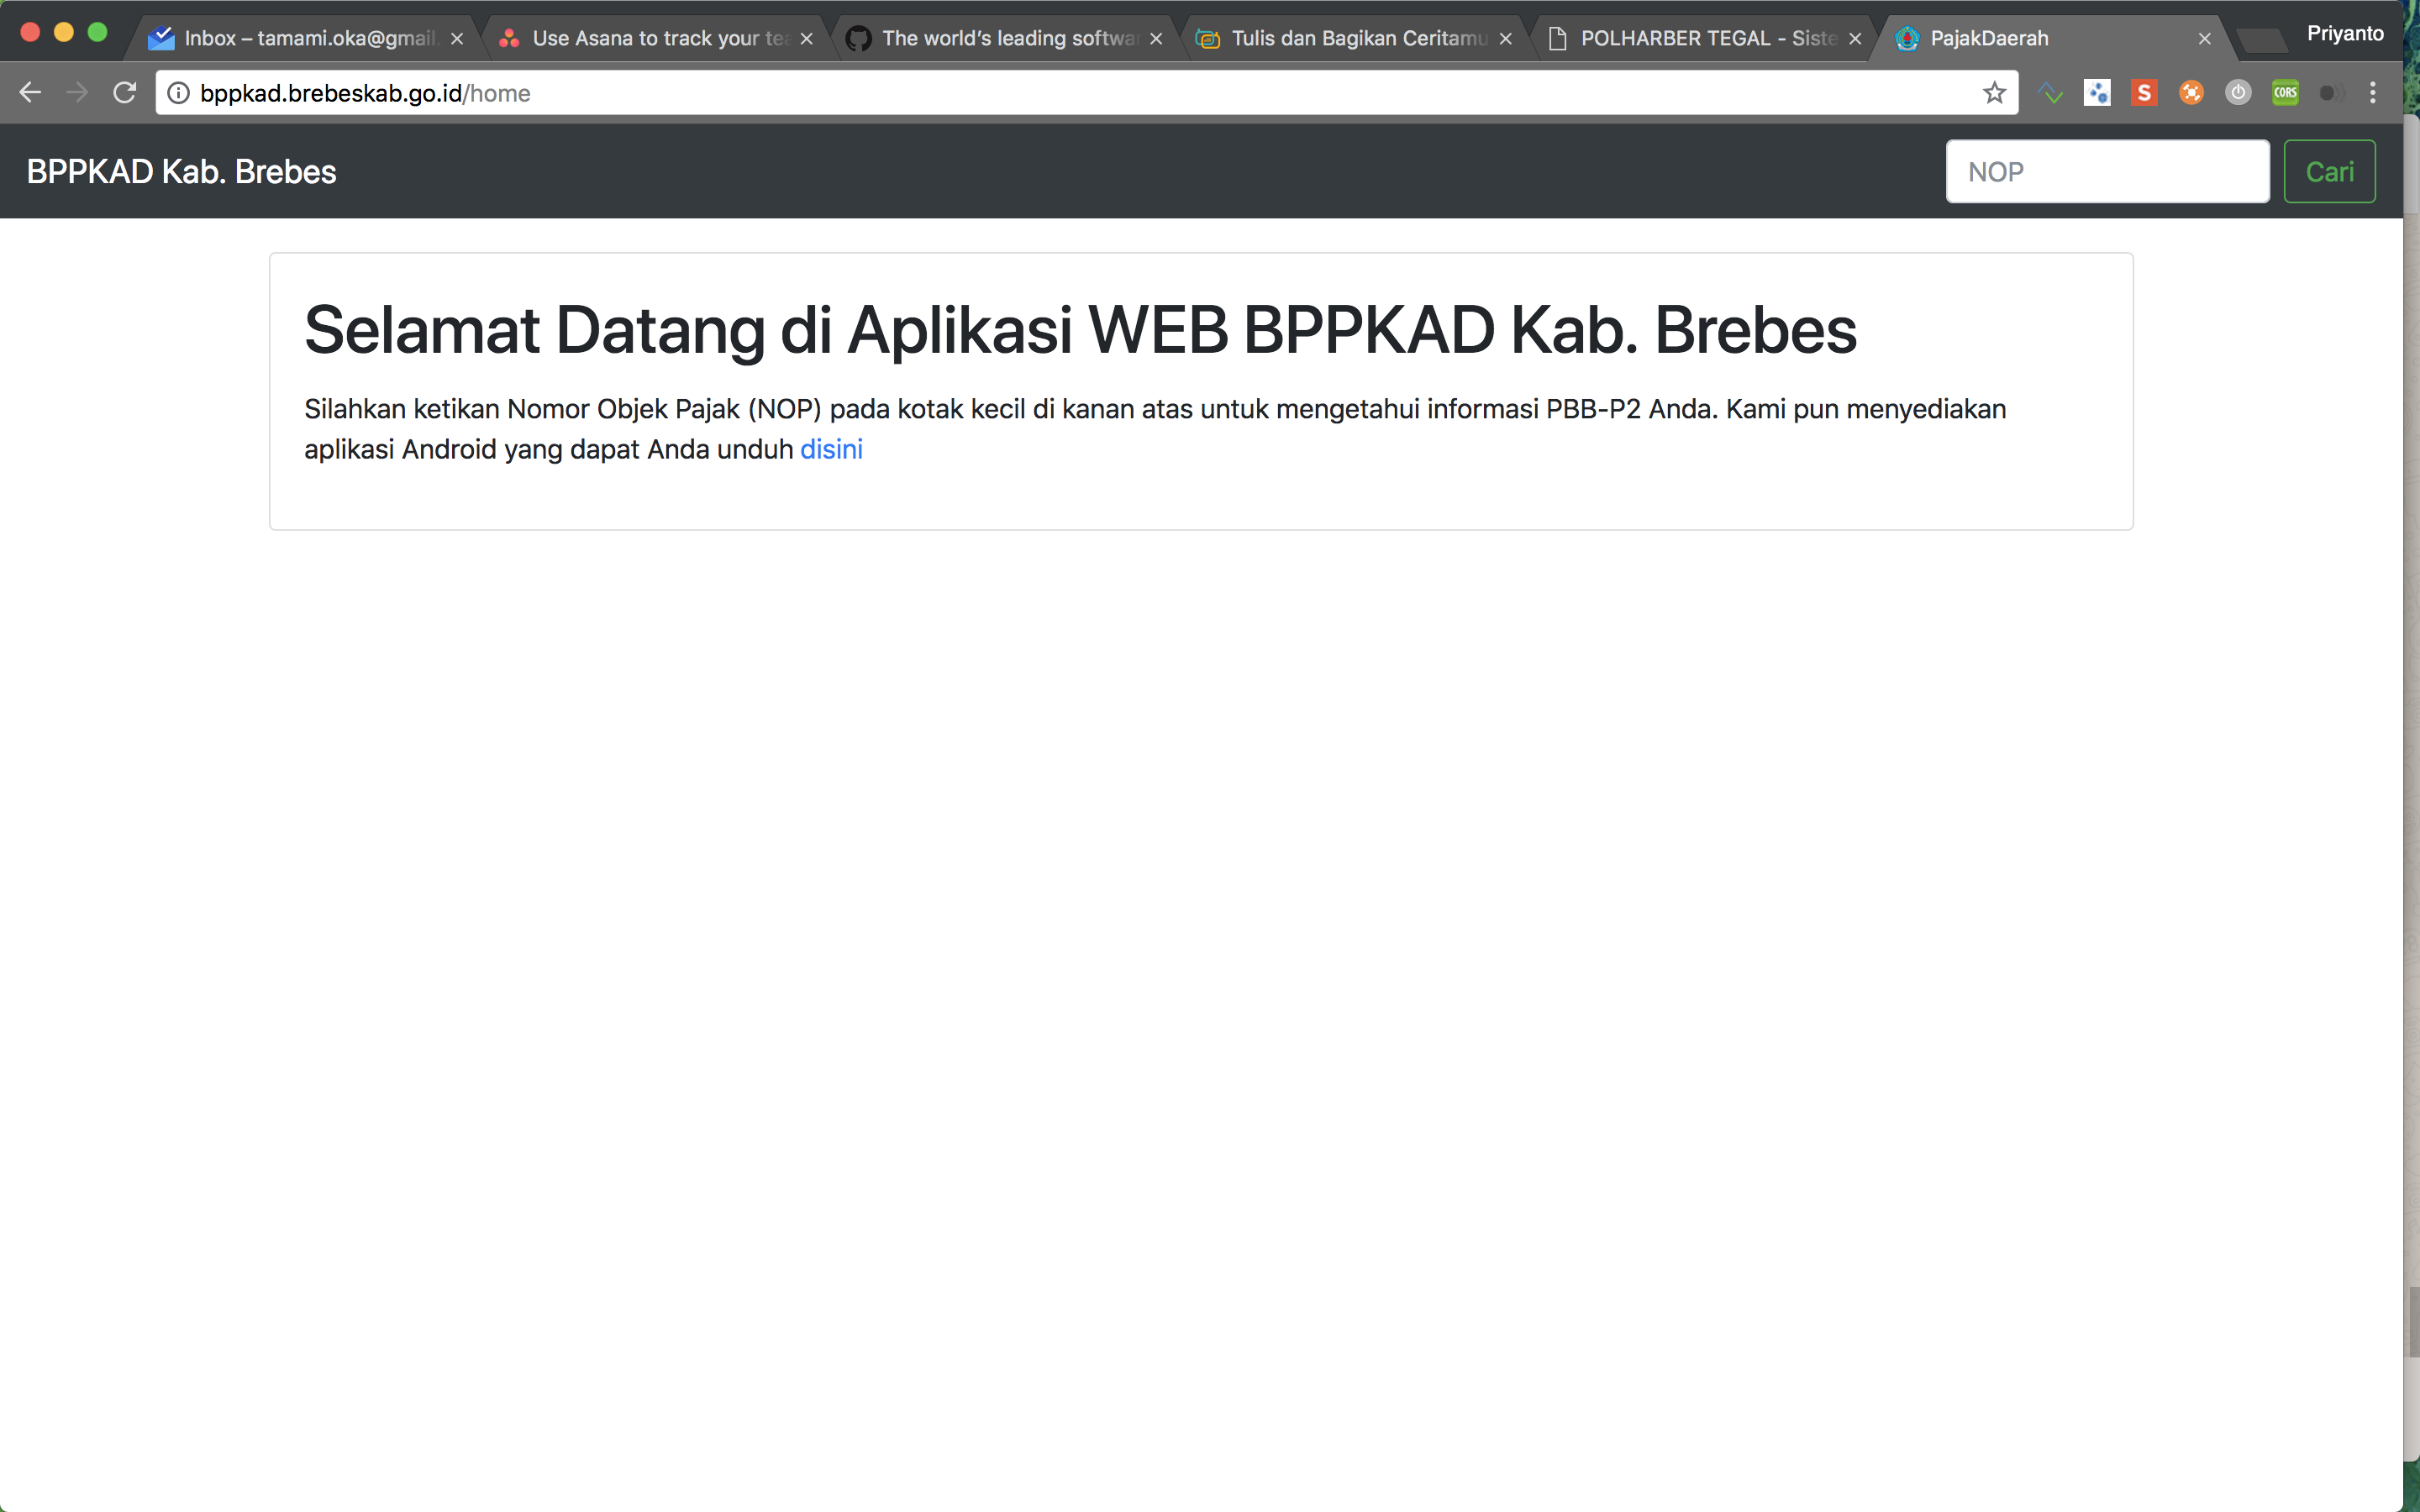
\includegraphics[width=1\textwidth]{./resources/main-fe}
	\caption{Tampilan Utama Aplikasi}
	\label{fig:main-fe}
\end{figure}

Pengguna tinggal memberikan Nomor objek Pajak (NOP) pada tempat yang telah disediakan di sebelah kanan atas halaman ini, Nomor Objek Pajak (NOP) adalah nomor yang tertera di sebelah kiri atas lembar Surat Pemberitahuan Pajak Terhutang (SPPT).

Aturan penulisan Nomor Objek Pajak (NOP) pada aplikasi ini tidak perlu menggunakan tanda baca seperti yang tertera pada lembar Surat Pemberitahuan Pajak Terhutang (SPPT), namun cukup untuk memasukkan atau mengetikkan angkanya saja, seperti contoh pada gambar \ref{fig:contoh-nop} berikut ini :

\begin{figure}[H]
	\centering
	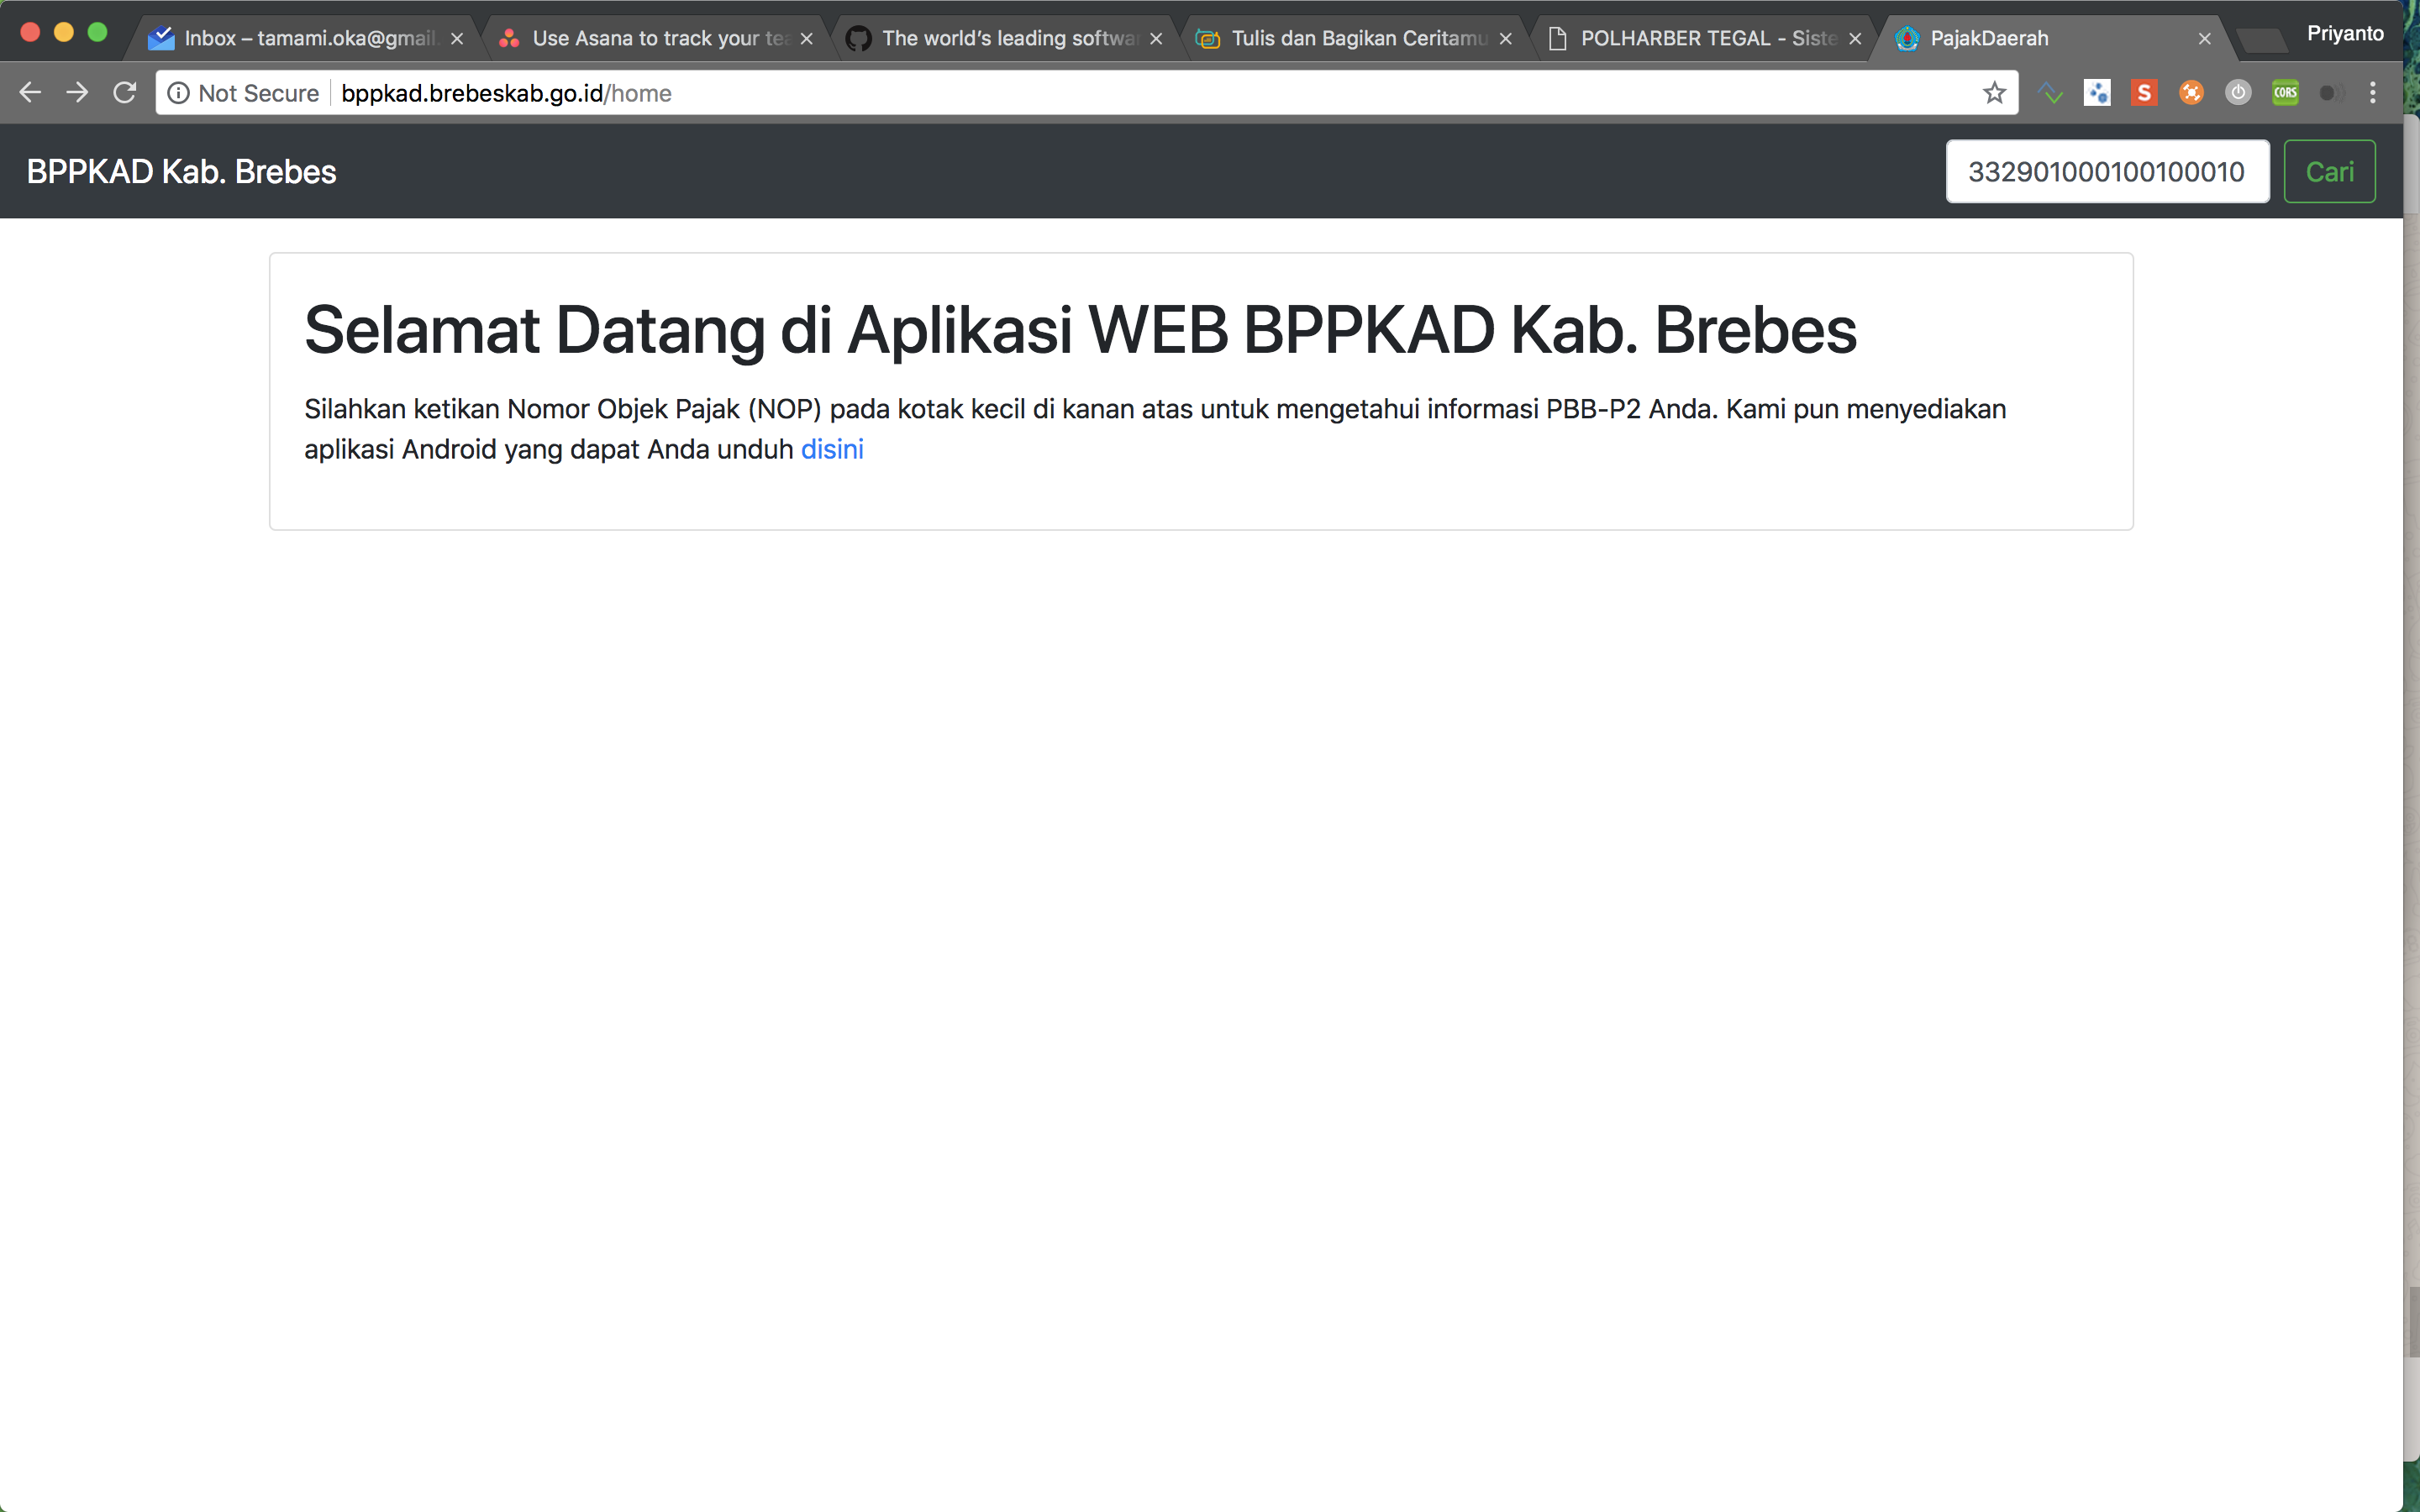
\includegraphics[width=1\textwidth]{./resources/contoh-input-nop}
	\caption{Contoh Memasukkan Nomor Objek Pajak (NOP)}
	\label{fig:contoh-nop}
\end{figure}

Setelah itu menekan tombol \textbf{Cari} di sebelahnya sehingga aplikasi akan menampilkan informasi mengenai objek pajak, subjek pajak, serta status tagihan dan pembayaran dari Surat Pemberitahuan Pajak Terhutang untuk tiap tahun pajaknya seperti gambar \ref{fig:result-info} berikut ini :

\begin{figure}[H]
	\centering
	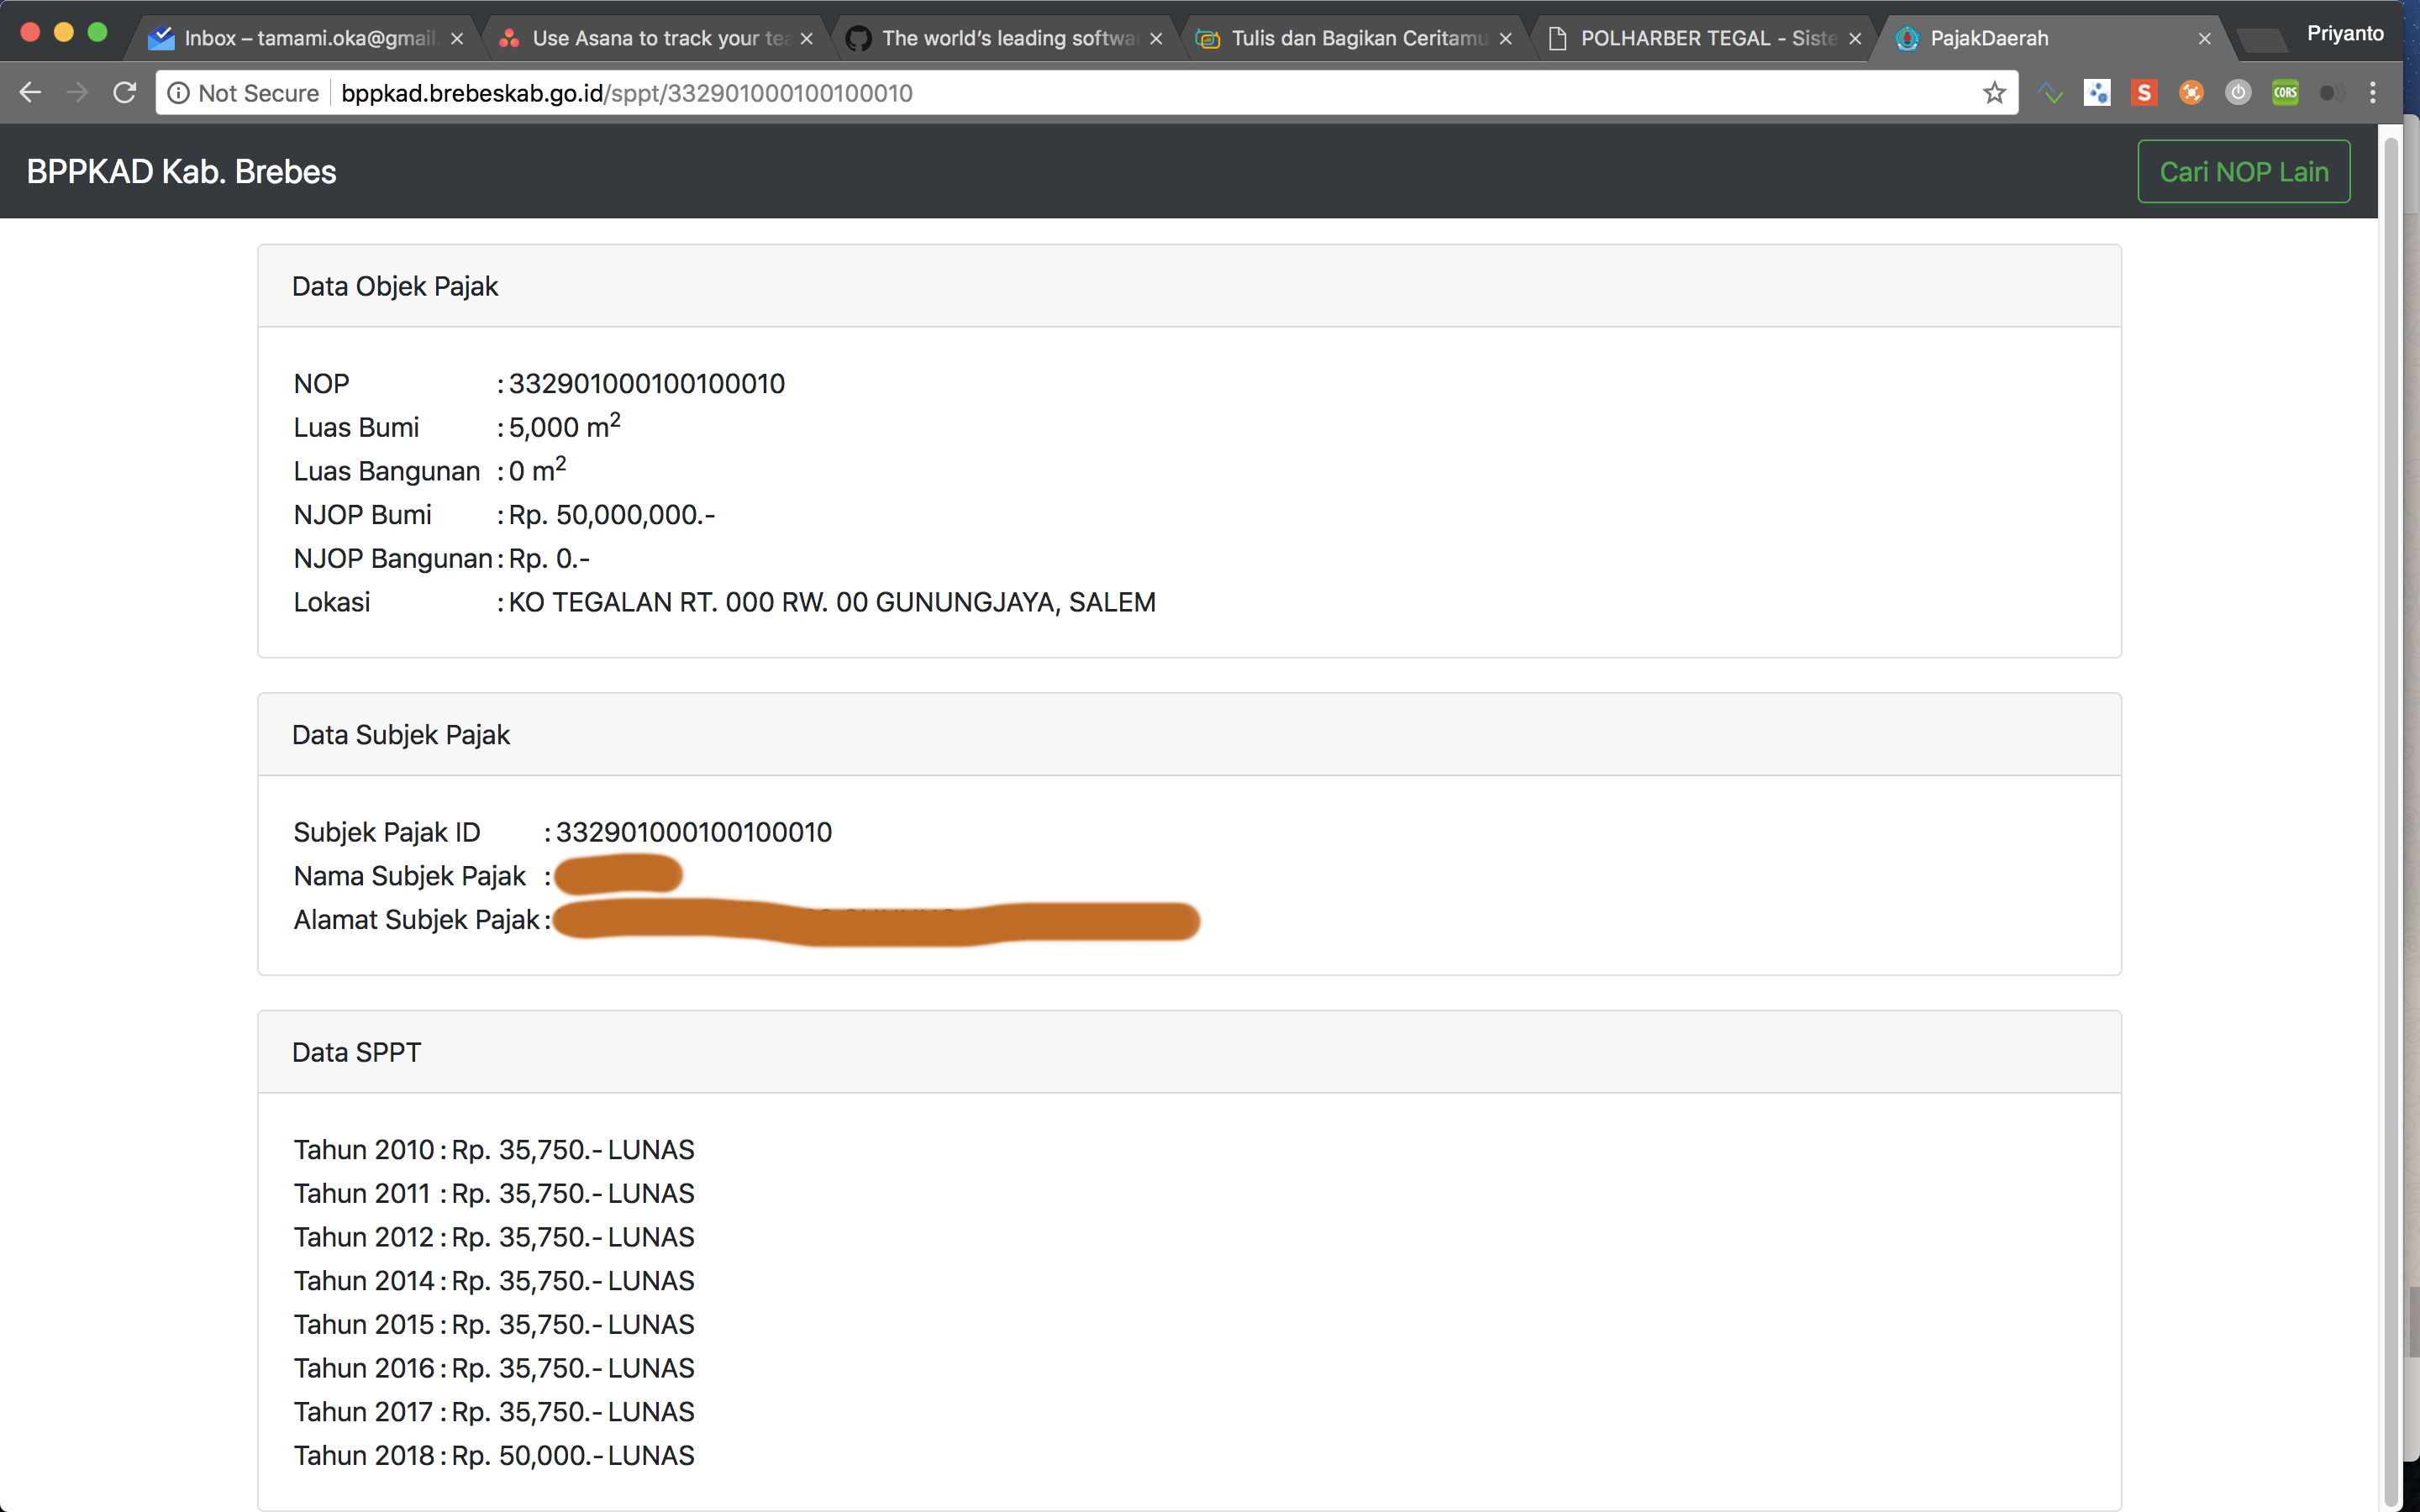
\includegraphics[width=1\textwidth]{./resources/result-info}
	\caption{Hasil Informasi Yang DIdapatkan}
	\label{fig:result-info}
\end{figure}


\backmatter%%%%%%%%%%%%%%%%%%%%%%%%%%%%%%%%%%%%%%%%%%%%%%%%%%%%%%%
\printindex

%%%%%%%%%%%%%%%%%%%%%%%%%%%%%%%%%%%%%%%%%%%%%%%%%%%%%%%%%%%%%%%%%%%%%%

\end{document}





